This section describes the three datasets used by the common evaluation framework. They are analysed separately so that the much larger PathVQA split does not dominate the other settings.

\section{Dataset Selection}

PathVQA provides a large histopathology benchmark, VQA-RAD changes the image domain to radiology, and ProstateMM-CHIMERA adds patient-linked clinical context to a prostate assessment task. Differences in image type, question form, answer length, and context allow the stability of model and detector rankings to be examined without treating any dataset as more important than another. The comparison tests dataset dependence; it does not prove clinical generalisation.

\begin{table}[htbp]
    \centering
    \caption{Dataset setting, unit of analysis, and evaluation size.}
    \label{tab:dataset-overview}
    \small
    \begin{tabularx}{\textwidth}{lXXr}
        \toprule
        Dataset & Image setting & Unit of analysis & Test records \\
        \midrule
        PathVQA & Histopathology & Image-question pair & 6,719 \\
        VQA-RAD & Radiology & Image-question pair & 451 \\
        ProstateMM-CHIMERA & Prostate assessment & Patient-linked task record & 42 \\
        \bottomrule
    \end{tabularx}
\end{table}

\section{PathVQA}

PathVQA contains pathology images with questions about organs, tissues, appearances, and disease-related concepts \citep{he2020pathvqa}. The experiment uses the complete official test split of 6,719 image-question pairs; no item is used for adaptation or model selection. Each record provides an image, question, and reference answer, and the same ordered records are evaluated by all three models. Figure~\ref{fig:pathvqa-example} illustrates the short, locally focused answer style and the potential difficulty of lexical evaluation when valid medical terms have different surface forms.

\begin{figure}[htbp]
    \centering
    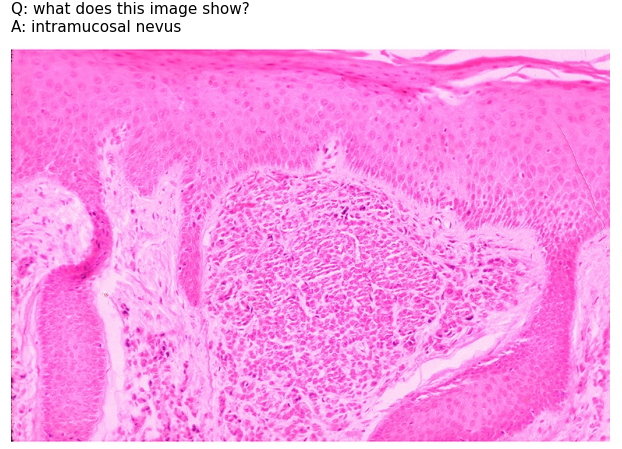
\includegraphics[width=0.82\textwidth]{Images/dataset_example_pathvqa.png}
    \caption[Representative PathVQA record]{Representative PathVQA record. Source: PathVQA \citep{he2020pathvqa}.}
    \label{fig:pathvqa-example}
\end{figure}

\section{VQA-RAD}

VQA-RAD contains radiology images with clinician-generated closed and open questions \citep{lau2018vqarad}. Its official test split contains 451 image-question pairs, all evaluated zero-shot with one greedy and three sampled answers. The modality, terminology, and answer distribution differ from PathVQA, making it a distinct test of the relationship between answer quality and failure detection. The smaller sample requires caution when interpreting close differences, and the dataset does not reproduce a complete radiology reporting workflow.
The final per-record exports were checked separately for this split. Each model file contains the same 451 indices (0--450), no empty greedy answers, and three sampled answers per item. The files use the model keys \texttt{qwen2\_5\_vl\_3b}, \texttt{llava\_1\_5\_7b}, and \texttt{medgemma\_4b\_it}; these keys are used to identify the final checkpoints in the analysis.

\begin{figure}[htbp]
    \centering
    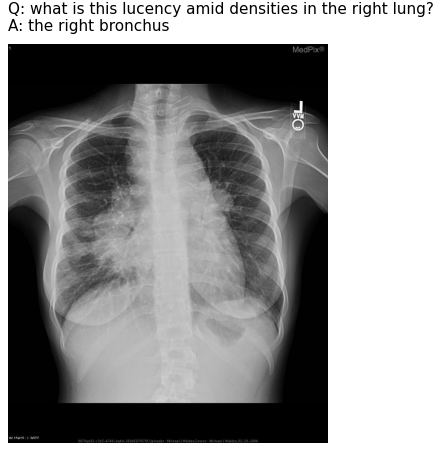
\includegraphics[width=0.74\textwidth]{Images/dataset_example_vqarad.png}
    \caption[Representative VQA-RAD record]{Representative VQA-RAD record. Source: VQA-RAD \citep{lau2018vqarad}.}
    \label{fig:vqarad-example}
\end{figure}

\section{ProstateMM-CHIMERA}

ProstateMM-CHIMERA is the project evaluation package derived from CHIMERA 2025 Task 1 on prostate cancer biochemical recurrence prediction \citep{chimera2025task1}; it is not presented as a separately published dataset under that exact name. Records combine histopathology, a focused question, and structured clinical context. The full package contains 285 task records from 95 patients, divided into 201 training, 42 validation, and 42 test records, with three records per patient. Only the held-out test records from 14 patients are used, so results are task-record estimates rather than independent patient-level estimates. Figure~\ref{fig:chimera-example} shows the more decision-oriented answer style.

\begin{figure}[htbp]
    \centering
    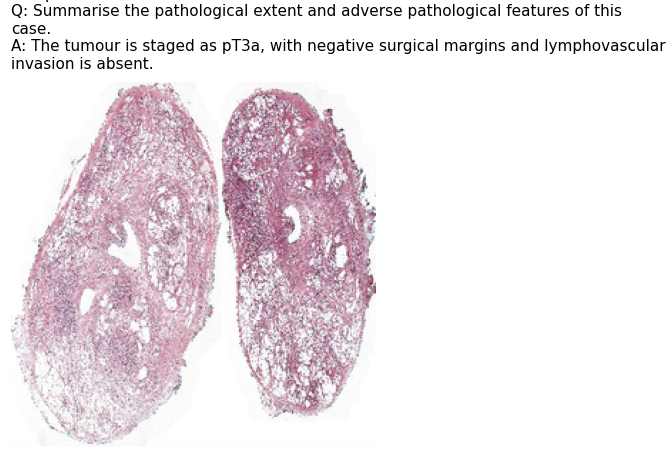
\includegraphics[width=0.82\textwidth]{Images/dataset_example_chimera.png}
    \caption[Representative ProstateMM-CHIMERA record]{Representative record from the project package derived from CHIMERA 2025 Task 1 \citep{chimera2025task1}.}
    \label{fig:chimera-example}
\end{figure}

\section{Prompts and Processing}

Each dataset uses one domain-specific prompt fixed across Qwen2.5-VL-3B-Instruct, LLaVA-1.5-7B, and MedGemma-4B-it. The prompts define the available evidence and request concise answers; ProstateMM-CHIMERA adds clinical context but excludes target facts and references from the model input.

\subsection{PathVQA Prompt}

\begin{quote}
You are a professional pathologist specialized in histopathology. You are answering visual questions based on pathology slide images. Use the given image, the question, and appropriate pathology knowledge to answer. For yes/no questions, answer only `yes' or `no'. For other questions, answer with the shortest medically appropriate phrase or term. Do not repeat the question. Do not provide explanations or unrelated information.
\end{quote}

\subsection{VQA-RAD Prompt}

\begin{quote}
You are a medical imaging specialist experienced in radiology. You are answering visual questions based on radiological images. Use the image, the question, and appropriate radiological knowledge to answer. For yes/no questions, answer only `yes' or `no'. For other questions, provide a concise radiological answer using a short phrase. Do not repeat the question. Do not add uncertain diagnosis, treatment advice, or unrelated details.
\end{quote}

\subsection{ProstateMM-CHIMERA Prompt}

\begin{quote}
You are a specialist pathologist experienced in prostate cancer assessment. You are answering visual questions based on prostate histopathology images and the provided clinical context. Use only the image, the question, and the clinical context to answer. For biochemical recurrence prediction or other yes/no questions, answer only `yes' or `no'. For grading, extent assessment, or other open-ended questions, answer with the most concise clinically appropriate phrase or value. Do not repeat the question. Do not provide long explanations, reasoning steps, or unrelated information.
\end{quote}

Generated text is cleaned by removing common assistant prefixes, normalising whitespace, and retaining the first non-empty line; case and punctuation are normalised only for scoring, and predictions are not rewritten to match references.

\section{Records and Data Quality}

The unit of analysis is an image-question pair for PathVQA and VQA-RAD and a patient-linked task record for ProstateMM-CHIMERA. All three models evaluate the same source records, producing 20,157 PathVQA, 1,353 VQA-RAD, and 126 ProstateMM-CHIMERA greedy model-item outputs, each paired with three samples. Source indices preserve joins between answers, labels, and detector scores. Image paths, required fields, splits, cache size, and duplicate records are checked before scoring; final PathVQA results use records marked \texttt{test\_full}, while ProstateMM-CHIMERA uses \texttt{test}. The complete VQA-RAD per-record exports permit direct calculation of failure prevalence, while coverage rows remain selective operating points rather than prevalence estimates. The small prostate test and within-patient dependence remain explicit limits.
